Several experiments on this supervised learning challenge have been conducted using a variety of different techniques for classification. The experiments are performed on the encoded data sets; \textit{FIN-Benthic} and an augmented version \textit{FIN-Benthic-Augmented} using the pair-wise information in the original data. The classification methods are; k-Nearest Neighbors (kNN), Linear Discriminant Analysis (LDA), Support Vector Machines (SVM), Perceptron and Neural Networks (NN). Commonly for all these supervised learning algorithm is the need for training. Training an algorithm is an optimization process of a loss criterion. The loss function explains the goodness of the model. Cross Validation (CV) are used for model selection to evaluate the best performing model. All the methods have been applied to the data sets on full dimensions and additionally with dimensionality reduction as a preprocessing step in the classification pipeline. Grid search have been used to search for good hyperparameters. Hyperparameters are user specified parameters that controls the algorithm's behavior \cite{Goodfellow-et-al-2016}. Hyperparameter search have been applied for all classifiers. Furthermore the degree of dimensionality reduction have been investigated in the same manner. Lastly existing Convolutional Neural Network architectures have been used on the raw images using the promise of transfer learning to use a pre-trained model to gain faster and better performing models on small data sets. For the transfer learning task the existing train, validation and test split have been used.

\paragraph{k-Nearest Neighbors (kNN)}

K-Nearest Neighbor is a distance-based classifier and as the name implies, classifies to the most common occurring class of the k-nearest neighbors \cite{karpathy}. There exist a variety of distance metrics, some example are; Euclidean, Minikowski and Manhattan distance \cite{AIML}. 

\begin{figure}[H]
    \centering
    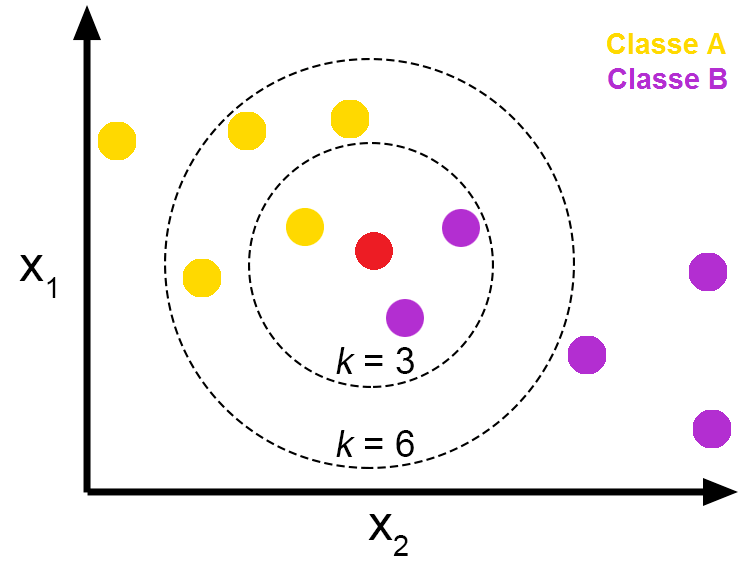
\includegraphics[width=0.4\textwidth]{figures/knn.png}
    \caption[]{k-Nearest Neighbor classifies the red sample to class B for $k=3$, however for $k=6$ it classifies to class A. Credits: Italo José}
    \label{fig:knn}
\end{figure}

\paragraph{Linear Discrmininat Analysis (LDA)}

Linear Discriminant Analysis is a linear transformation of the data. The linear transformation is an optimization, that tries to maximize the distance between classes and minimize the distance within a class\cite{AIML}. Figure \ref{fig:lda_dec} shows how LDA discriminates two classes.

\begin{figure}[H]
    \centering
    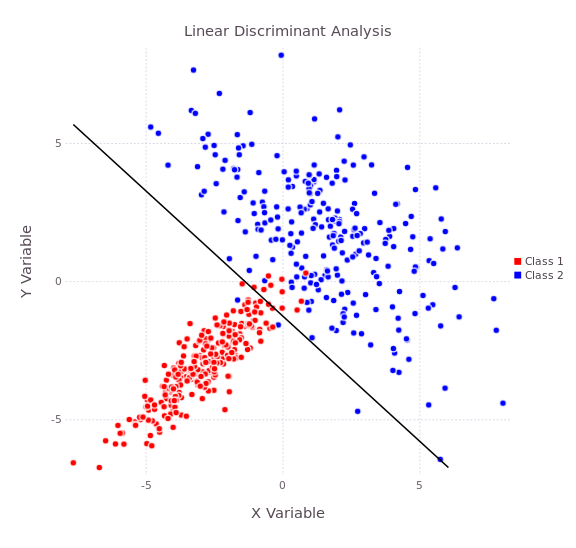
\includegraphics[width=0.4\textwidth]{figures/lda_deci.png}
    \caption[]{LDA creates a linear decision function. The linear decision function is a decision hyperplane which discriminates classes. Credits: Tim Thatcher}
    \label{fig:lda_dec}
\end{figure}

LDA can also be used for dimensionality reduction, this would be further explained later.

\paragraph{Support Vector Machine (SVM)}

SVM can be used for classification. SVM tries to find the decision hyperplanes, that maximizes th distance between classes \cite{IR}. The decision hyperplane are given by a linear function $w^Tx+b$, when the function is positive it predicts the class to be present, and intuitively the class is not present, when the function is negative \cite{Goodfellow-et-al-2016}. The Support Vector Machine uses support vectors to define the decision hyperplane. The support vectors are vectors of the training data, that maximizes the margin between to classes. The original SVM proposed by Boser et al. \cite{Boser} utilized a hard-margin. The hard-margin is the optimal decision hyperplane, however it only works well when the data is linearly separable. Vapnik et al. \cite{Vapnik} proposed a soft-margin, which is more robust to noise by introducing some slack i the fom of the hinge loss function.

One of the most promising contribution associated with SVMs is the kernel trick. The kernel trick makes not only SVM useful when data is not linearly separable, but all machine learning algorithms, that can be rewritten exclusively in terms of dot product between examples. The kernel trick is a mapping of the data into a higher dimensional space - even with indefinite dimensions. The kernel trick is equivalent to transforming all data points into higher dimensions, but with a lot less computational demands. In the high dimensional space a linear decision boundary can be obtained. One of the most widely used kernels are the gaussian kernel or radial basis function (RBF), which maps to an indefinite dimensional space \cite{Goodfellow-et-al-2016}.

\begin{figure}[H]
    \centering
    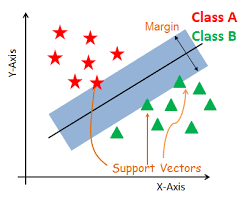
\includegraphics[width=0.4\textwidth]{figures/svm.png}
    \caption[]{A binary SVM constructing the decision hyperplane, that maximizes the margin between the support vectors of the two classes. Credits: Avinash Navlani}
    \label{fig:svm}
\end{figure}

\paragraph{Perceptron}

Perceptrons is a single layer Neural Network. The perceptron was set forth by Frank Rosenblatt \cite{Perceptron}, as a way of mimicking human perception. Perceptrons produces a linear decision function and only performs well on linearly separable data. 

\begin{figure}[H]
    \centering
    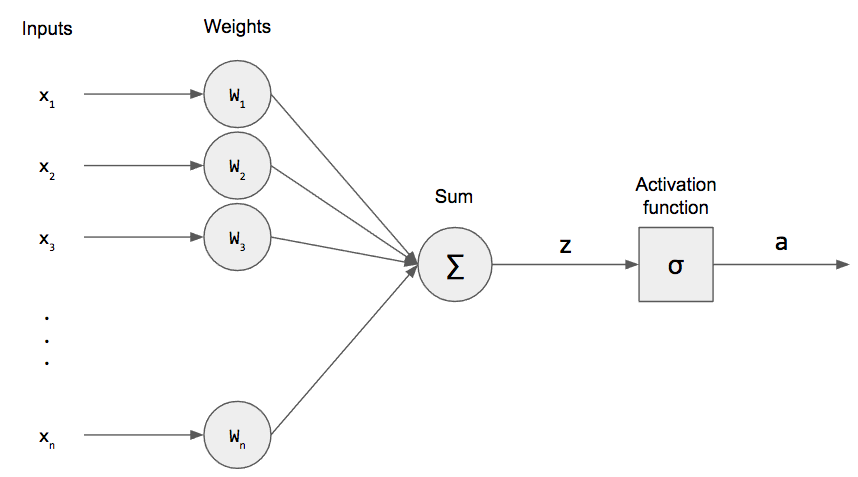
\includegraphics[width=0.4\textwidth]{figures/perceptron.png}
    \caption[]{The perceptron takes a feature vector as input. All the feature are multiplied by a weight. The weight are then summed to what is called a weighted sum. An activation function are applied to the weighted sum. The output of the activation function is the classification. Credits: Stanley Obumneme Dukor}
    \label{fig:perc}
\end{figure}

The perceptron are trained by iteratively updating the weights to produce the correct output for the training data. The loss function are rather simple, if the sample is correctly classified th loss function will output zero and it will output 1 if misclassified. This means the perceptron's weight are only updated when is fails to classify a sample. 

\paragraph{Neural Network (NN)}

Neural Networks extends the perceptron. This ideas was sparked by progress within biology, that mapped human perceptions into a network of neurons i.e. perceptrons. The first working Artificial Neural Network (ANN or NN) was completed by A. G. Ivakhnenko and V. G. Lapa \cite{Alexey}. The perceptrons where extended by adding more layers between input and output referred to as hidden layers. The NN is capable of producing non-linear decision functions, thus overcomes the short comings of the perceptron.  

\begin{figure}[H]
    \centering
    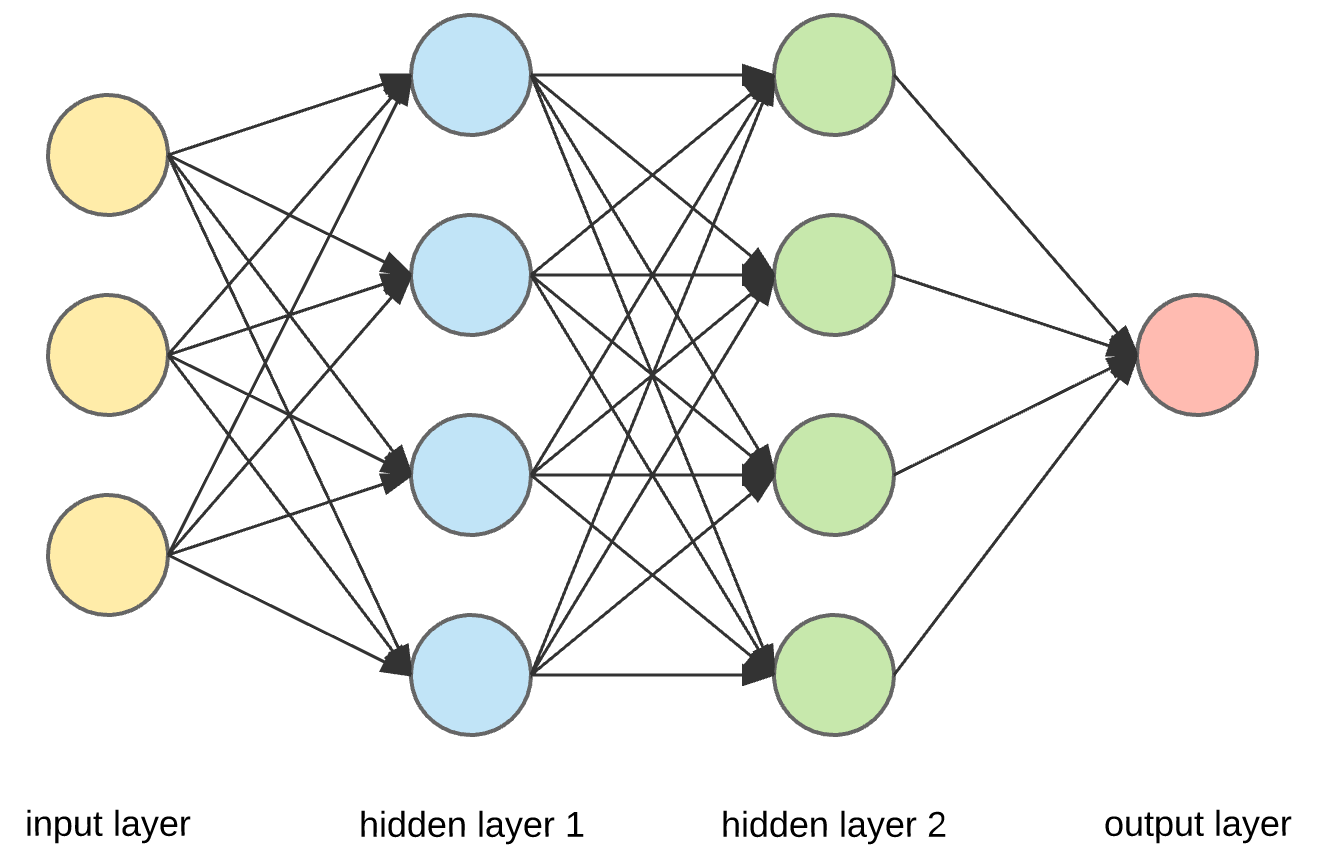
\includegraphics[width=0.4\textwidth]{figures/nn.png}
    \caption[]{Neural Network with two hidden layers. Each layer is formed by a number of neurons. A fully-connected dense neural network receives all output from previous layer as input. The input are multiplied by the neuron's weight and a bias is added. At last the non-linear activation function is applied. Credits: Arden Dertat}
    \label{fig:nn}
\end{figure}

Training a NN is way more complex than a perceptron. The training are done using feed-forward and back-propagation. Training vectors are given to the network, where all nodes do their operations upon reception. The output from this layers are then fed forward to the next layer. When it reaches the end of the network an error term is computed using the loss function. The error are then back-propagated throughout the network, where the nodes' contribution to the error is computed. Using gradients the network's weights are optimized. 

\paragraph{Convolutional Neural Network (CNN)}

CNNs are today the golden standard to obtain good classification results on images. AlexNet was the first CNN, that made a breaking result on the ImageNet Challenge in 2012. Since then a lot of then architectures have been proposed and introducing smaller changes to improve just a little is published every now and then. Traditional neural network does not scale to task as images increases in size. CNNs' does not take single pixels as input, but instead convolutional layers are added to the architecture to inspect local regions of pixels to accommodate spatial correlation in images also known as filters. The network then learns filters, that represents features such as a diagonal edge, a blob, etc. Throughout the network the image is down sampled by pooling layers and eventually classified using typically a softmax layer \cite{karpathy-convnet}. 

\begin{figure}[H]
    \centering
    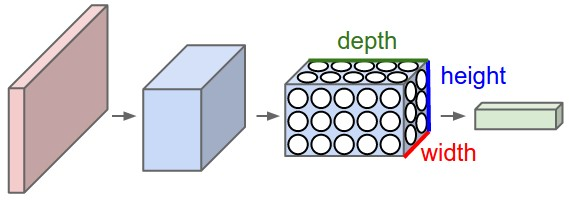
\includegraphics[width=0.4\textwidth]{figures/cnn.jpeg}
    \caption[]{A CNN arranges its neurons in three dimensions. The layers of the CNN transforms the 3D input to a 3D output of neuron activations. The input layer holds the image and the width and height equals the dimensions of the image, and the depth equals 3 i.e. the color channels 'RGB' of the image. Credits: Andrej Karpathy}
    \label{fig:cnn}
\end{figure}

GoogleNetV4 aka. InceptionResNetV2 \cite{SzegedyIV16} is a very deep CNN, in fact 572 layers deep. It is one of the top-scoring networks on the ImageNet Challenge with a top-5 accuracy equalling 0.95. \cite{chollet} It is available trough Keras with pre-trained ImageNet weights. 

This sums of all the classification methods used in this paper. Next I describe practices concerning machine learning.

\paragraph{Dimensionality Reduction}

Dimensionality reduction as the name implies down scales the feature space into a lower dimensional space. The techniques used in this paper is the already covered LDA and Principal Component Analysis (PCA).

\subparagraph{Principal Component Analysis (PCA)}

PCA is an unsupervised learning technique. It learns an orthogonal linear transformation onto a smaller feature space. The number of dimensions i.e. principal components are a hyperparameter. PCA tries to preserve as much as the information i.e. variance as possible. The first component i.e. dimension is a projection a long the axis of the data with the most variance, the second component is orthogonal to the first component and describes the axis with the second most variance. The third component then describes the axis with third most variance and so on. The figure \ref{fig:pca} the component axis as vector called $PC1$ and $PC2$.

\begin{figure}[H]
    \centering
    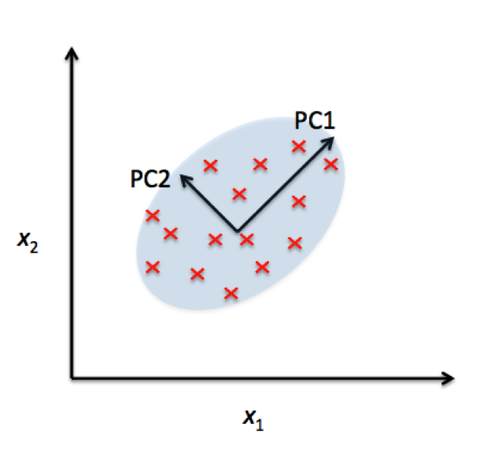
\includegraphics[width=0.4\textwidth]{figures/pca.png}
    \caption[]{Principal Component Analysis in a 2 dimensional space. PCA rotates the data to be perpendicular to the principal components axises. Credits: Sebastian Raschka}
    \label{fig:pca}
\end{figure}

\subparagraph{Linear Discriminant Analysis (LDA)}
As mention LDA can be used for dimensionality reduction as well. One must specify the $n$ number of components i.e. dimensions to transform the data onto, if the $n$ are less than the original data dimensions D, then the number of dimensions will be reduced. 

\begin{figure}[H]
    \centering
    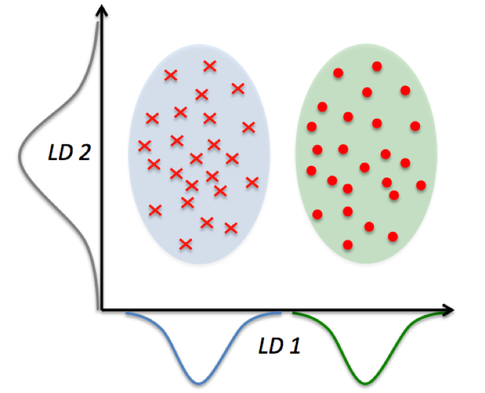
\includegraphics[width=0.4\textwidth]{figures/lda.png}
    \caption[]{Linear Discriminant Analysis project the data onto and axis, that maximize the distance between the classes and minimizes the distance within the respective classes. LD1 is a good project, whereas LD1 is not. Credits: Sebastian Raschka}
    \label{fig:lda}
\end{figure}

\paragraph{Model Selection}

Model selection covers procedures to train the best model and avoid overfitting the model to the training data. Overfitting is the pitfall of having a model, that describes the training data too well, thus suffers not to generalize the true underlying structure of the data. Although other methods exists the two used in this paper are Validation Holdout and Cross Validation. 

\subparagraph{Validation Holdout}

Validation Holdout takes a fraction of your available labelled data and hold it out of the training procedure. 

\begin{figure}[H]
    \centering
    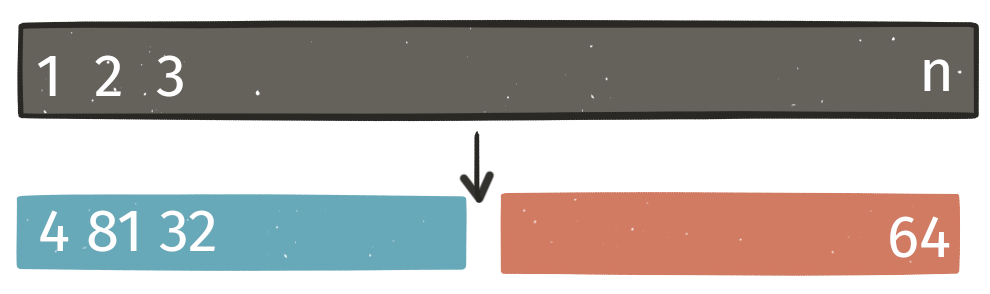
\includegraphics[width=0.4\textwidth]{figures/validationset.png}
    \caption[]{The validation subset is then used to validate the model's performance on data it has not been training.}
    \label{fig:val_holdout}
\end{figure}

The assumption is that the holdout set resembles the true data, since it has been drawn from the same distribution \cite{Goodfellow-et-al-2016}. If the model performs well on both training and validation it is assumed to be a good model. The split is typically made $70/30$ or $80/20$ for training data and validation data respectively. 

\subparagraph{Cross Validation (CV)}

Cross Validation extends on the holdout validation. $k$-fold Cross Validation create $k$ experiments compared to one. The entire data set are split in $k$ folds, for every $k$ step one subset is for validation and the remaining $k-1$ fold are used for training \cite{Goodfellow-et-al-2016}. Figure \ref{fig:cv} illustrates the idea. 

\begin{figure}[H]
    \centering
    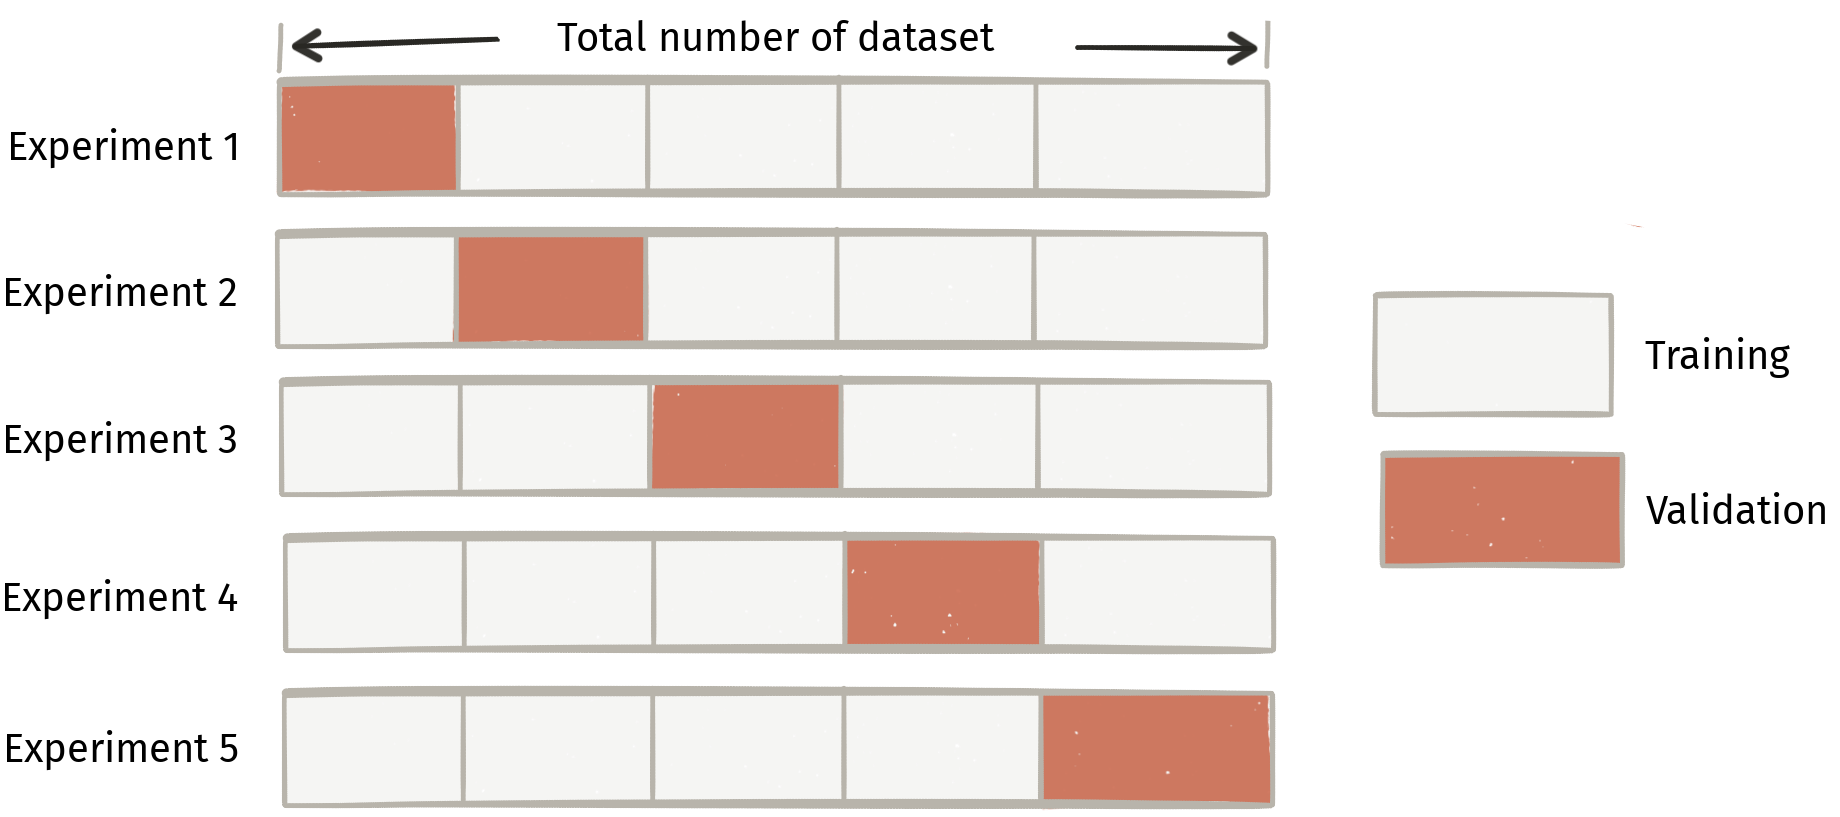
\includegraphics[width=0.5\textwidth]{figures/cv.png}
    \caption[]{Cross Validation ensures that the model have been trained on all the data and validated as well. The selection folds are typically either $k=5$ or $k=10$. }
    \label{fig:cv}
\end{figure}

\paragraph{Hyperparameter Search}

There are mainly two approaches to search for hyperparameters; Random Search and Grid Search other than heuristic guessing. In this paper Grid Search are used.

\subparagraph{Grid Search}

Grid Search is an approach to seek better hyperparameters for your model. You specify a set of options for all hyperparameters and then search all possible combinations in the grid. 

\begin{figure}[H]
    \centering
    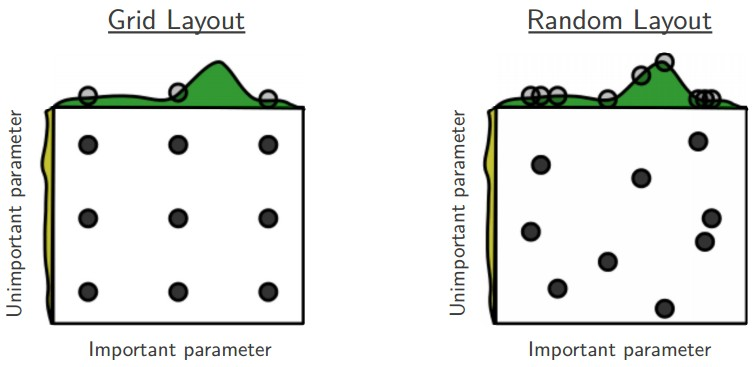
\includegraphics[width=0.4\textwidth]{figures/gridsearch_vs_randomsearch.jpeg}
    \caption[]{Grid search is a systematic approach to explore a broader space of hyperparameters although at the cost of additional time. The down-side of this approach is, that it is still based on intuition of good hyperparameters. The random approach are also widely used and might be preferred, as it may find a sweet spot, that goes beyond human intuition, however that is no guarantee, and it is still time costly \cite{Bergstra}. Credits: Bergstra and Bengio}
    \label{fig:gs_vs_rs}
\end{figure}

  